\documentclass[1p]{elsarticle_modified}
%\bibliographystyle{elsarticle-num}

%\usepackage[colorlinks]{hyperref}
%\usepackage{abbrmath_seonhwa} %\Abb, \Ascr, \Acal ,\Abf, \Afrak
\usepackage{amsfonts}
\usepackage{amssymb}
\usepackage{amsmath}
\usepackage{amsthm}
\usepackage{scalefnt}
\usepackage{amsbsy}
\usepackage{kotex}
\usepackage{caption}
\usepackage{subfig}
\usepackage{color}
\usepackage{graphicx}
\usepackage{xcolor} %% white, black, red, green, blue, cyan, magenta, yellow
\usepackage{float}
\usepackage{setspace}
\usepackage{hyperref}

\usepackage{tikz}
\usetikzlibrary{arrows}

\usepackage{multirow}
\usepackage{array} % fixed length table
\usepackage{hhline}

%%%%%%%%%%%%%%%%%%%%%
\makeatletter
\renewcommand*\env@matrix[1][\arraystretch]{%
	\edef\arraystretch{#1}%
	\hskip -\arraycolsep
	\let\@ifnextchar\new@ifnextchar
	\array{*\c@MaxMatrixCols c}}
\makeatother %https://tex.stackexchange.com/questions/14071/how-can-i-increase-the-line-spacing-in-a-matrix
%%%%%%%%%%%%%%%

\usepackage[normalem]{ulem}

\newcommand{\msout}[1]{\ifmmode\text{\sout{\ensuremath{#1}}}\else\sout{#1}\fi}
%SOURCE: \msout is \stkout macro in https://tex.stackexchange.com/questions/20609/strikeout-in-math-mode

\newcommand{\cancel}[1]{
	\ifmmode
	{\color{red}\msout{#1}}
	\else
	{\color{red}\sout{#1}}
	\fi
}

\newcommand{\add}[1]{
	{\color{blue}\uwave{#1}}
}

\newcommand{\replace}[2]{
	\ifmmode
	{\color{red}\msout{#1}}{\color{blue}\uwave{#2}}
	\else
	{\color{red}\sout{#1}}{\color{blue}\uwave{#2}}
	\fi
}

\newcommand{\Sol}{\mathcal{S}} %segment
\newcommand{\D}{D} %diagram
\newcommand{\A}{\mathcal{A}} %arc


%%%%%%%%%%%%%%%%%%%%%%%%%%%%%5 test

\def\sl{\operatorname{\textup{SL}}(2,\Cbb)}
\def\psl{\operatorname{\textup{PSL}}(2,\Cbb)}
\def\quan{\mkern 1mu \triangleright \mkern 1mu}

\theoremstyle{definition}
\newtheorem{thm}{Theorem}[section]
\newtheorem{prop}[thm]{Proposition}
\newtheorem{lem}[thm]{Lemma}
\newtheorem{ques}[thm]{Question}
\newtheorem{cor}[thm]{Corollary}
\newtheorem{defn}[thm]{Definition}
\newtheorem{exam}[thm]{Example}
\newtheorem{rmk}[thm]{Remark}
\newtheorem{alg}[thm]{Algorithm}

\newcommand{\I}{\sqrt{-1}}
\begin{document}

%\begin{frontmatter}
%
%\title{Boundary parabolic representations of knots up to 8 crossings}
%
%%% Group authors per affiliation:
%\author{Yunhi Cho} 
%\address{Department of Mathematics, University of Seoul, Seoul, Korea}
%\ead{yhcho@uos.ac.kr}
%
%
%\author{Seonhwa Kim} %\fnref{s_kim}}
%\address{Center for Geometry and Physics, Institute for Basic Science, Pohang, 37673, Korea}
%\ead{ryeona17@ibs.re.kr}
%
%\author{Hyuk Kim}
%\address{Department of Mathematical Sciences, Seoul National University, Seoul 08826, Korea}
%\ead{hyukkim@snu.ac.kr}
%
%\author{Seokbeom Yoon}
%\address{Department of Mathematical Sciences, Seoul National University, Seoul, 08826,  Korea}
%\ead{sbyoon15@snu.ac.kr}
%
%\begin{abstract}
%We find all boundary parabolic representation of knots up to 8 crossings.
%
%\end{abstract}
%\begin{keyword}
%    \MSC[2010] 57M25 
%\end{keyword}
%
%\end{frontmatter}

%\linenumbers
%\tableofcontents
%
\newcommand\colored[1]{\textcolor{white}{\rule[-0.35ex]{0.8em}{1.4ex}}\kern-0.8em\color{red} #1}%
%\newcommand\colored[1]{\textcolor{white}{ #1}\kern-2.17ex	\textcolor{white}{ #1}\kern-1.81ex	\textcolor{white}{ #1}\kern-2.15ex\color{red}#1	}

{\Large $\underline{12a_{1028}~(K12a_{1028})}$}

\setlength{\tabcolsep}{10pt}
\renewcommand{\arraystretch}{1.6}
\vspace{1cm}\begin{tabular}{m{100pt}>{\centering\arraybackslash}m{274pt}}
\multirow{5}{120pt}{
	\centering
	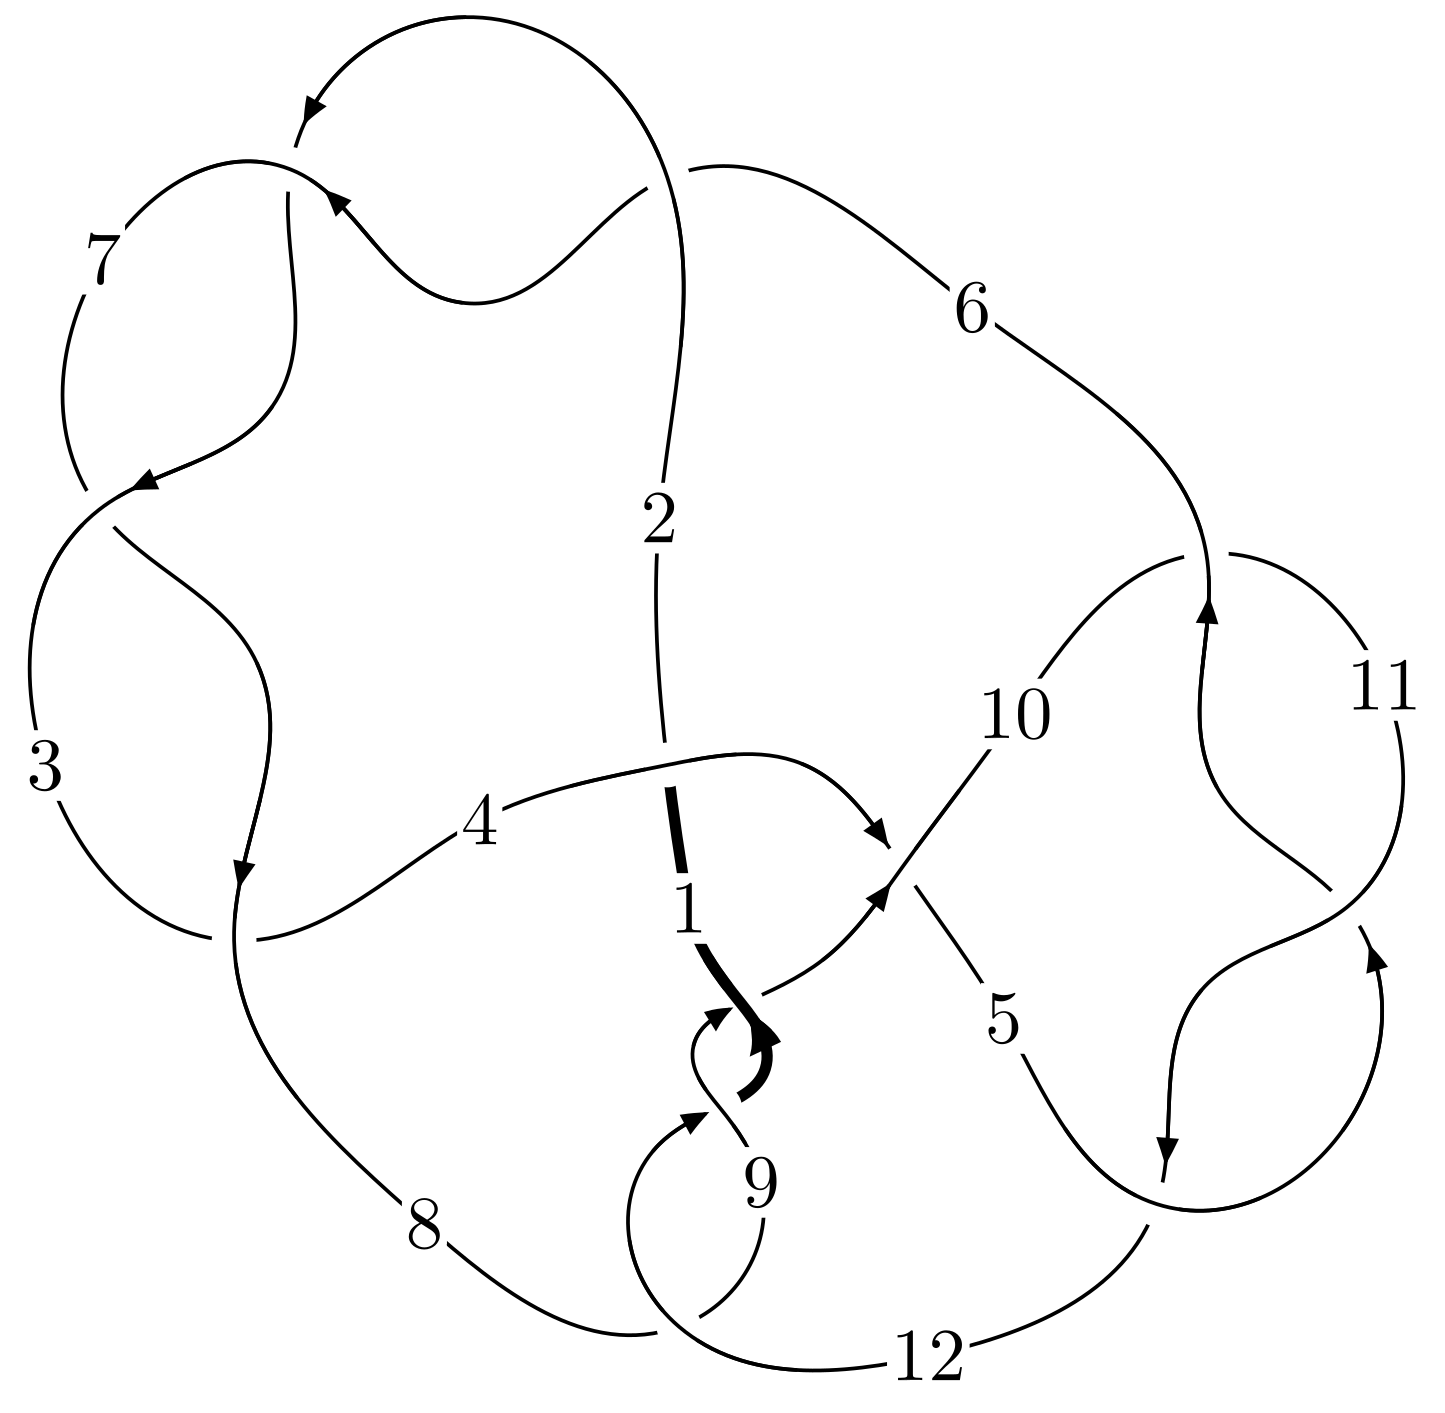
\includegraphics[width=112pt]{../../../GIT/diagram.site/Diagrams/png/1829_12a_1028.png}\\
\ \ \ A knot diagram\footnotemark}&
\allowdisplaybreaks
\textbf{Linearized knot diagam} \\
\cline{2-2}
 &
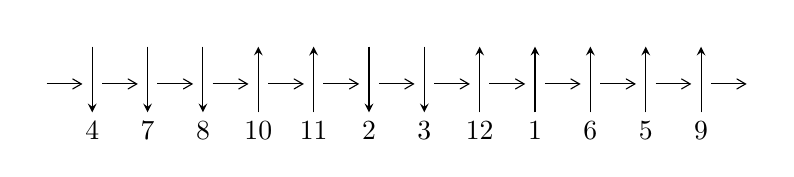
\begin{tikzpicture}[x=20pt, y=17pt]
	% nodes
	\node (C0) at (0, 0) {};
	\node (C1) at (1, 0) {};
	\node (C1U) at (1, +1) {};
	\node (C1D) at (1, -1) {4};

	\node (C2) at (2, 0) {};
	\node (C2U) at (2, +1) {};
	\node (C2D) at (2, -1) {7};

	\node (C3) at (3, 0) {};
	\node (C3U) at (3, +1) {};
	\node (C3D) at (3, -1) {8};

	\node (C4) at (4, 0) {};
	\node (C4U) at (4, +1) {};
	\node (C4D) at (4, -1) {10};

	\node (C5) at (5, 0) {};
	\node (C5U) at (5, +1) {};
	\node (C5D) at (5, -1) {11};

	\node (C6) at (6, 0) {};
	\node (C6U) at (6, +1) {};
	\node (C6D) at (6, -1) {2};

	\node (C7) at (7, 0) {};
	\node (C7U) at (7, +1) {};
	\node (C7D) at (7, -1) {3};

	\node (C8) at (8, 0) {};
	\node (C8U) at (8, +1) {};
	\node (C8D) at (8, -1) {12};

	\node (C9) at (9, 0) {};
	\node (C9U) at (9, +1) {};
	\node (C9D) at (9, -1) {1};

	\node (C10) at (10, 0) {};
	\node (C10U) at (10, +1) {};
	\node (C10D) at (10, -1) {6};

	\node (C11) at (11, 0) {};
	\node (C11U) at (11, +1) {};
	\node (C11D) at (11, -1) {5};

	\node (C12) at (12, 0) {};
	\node (C12U) at (12, +1) {};
	\node (C12D) at (12, -1) {9};
	\node (C13) at (13, 0) {};

	% arrows
	\draw[->,>={angle 60}]
	(C0) edge (C1) (C1) edge (C2) (C2) edge (C3) (C3) edge (C4) (C4) edge (C5) (C5) edge (C6) (C6) edge (C7) (C7) edge (C8) (C8) edge (C9) (C9) edge (C10) (C10) edge (C11) (C11) edge (C12) (C12) edge (C13) ;	\draw[->,>=stealth]
	(C1U) edge (C1D) (C2U) edge (C2D) (C3U) edge (C3D) (C4D) edge (C4U) (C5D) edge (C5U) (C6U) edge (C6D) (C7U) edge (C7D) (C8D) edge (C8U) (C9D) edge (C9U) (C10D) edge (C10U) (C11D) edge (C11U) (C12D) edge (C12U) ;
	\end{tikzpicture} \\
\hhline{~~} \\& 
\textbf{Solving Sequence} \\ \cline{2-2} 
 &
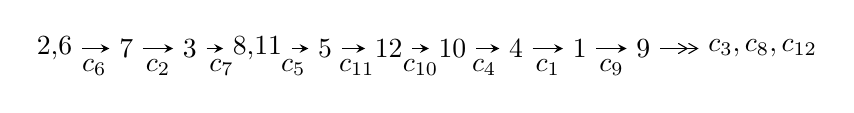
\begin{tikzpicture}[x=23pt, y=7pt]
	% node
	\node (A0) at (-1/8, 0) {2,6};
	\node (A1) at (1, 0) {7};
	\node (A2) at (2, 0) {3};
	\node (A3) at (49/16, 0) {8,11};
	\node (A4) at (33/8, 0) {5};
	\node (A5) at (41/8, 0) {12};
	\node (A6) at (49/8, 0) {10};
	\node (A7) at (57/8, 0) {4};
	\node (A8) at (65/8, 0) {1};
	\node (A9) at (73/8, 0) {9};
	\node (C1) at (1/2, -1) {$c_{6}$};
	\node (C2) at (3/2, -1) {$c_{2}$};
	\node (C3) at (5/2, -1) {$c_{7}$};
	\node (C4) at (29/8, -1) {$c_{5}$};
	\node (C5) at (37/8, -1) {$c_{11}$};
	\node (C6) at (45/8, -1) {$c_{10}$};
	\node (C7) at (53/8, -1) {$c_{4}$};
	\node (C8) at (61/8, -1) {$c_{1}$};
	\node (C9) at (69/8, -1) {$c_{9}$};
	\node (A10) at (11, 0) {$c_{3},c_{8},c_{12}$};

	% edge
	\draw[->,>=stealth]	
	(A0) edge (A1) (A1) edge (A2) (A2) edge (A3) (A3) edge (A4) (A4) edge (A5) (A5) edge (A6) (A6) edge (A7) (A7) edge (A8) (A8) edge (A9) ;
	\draw[->>,>={angle 60}]	
	(A9) edge (A10);
\end{tikzpicture} \\ 

\end{tabular} \\

\footnotetext{
The image of knot diagram is generated by the software ``\textbf{Draw programme}" developed by Andrew Bartholomew(\url{http://www.layer8.co.uk/maths/draw/index.htm\#Running-draw}), where we modified some parts for our purpose(\url{https://github.com/CATsTAILs/LinksPainter}).
}\phantom \\ \newline 
\centering \textbf{Ideals for irreducible components\footnotemark of $X_{\text{par}}$} 
 
\begin{align*}
I^u_{1}&=\langle 
-1.85413\times10^{21} u^{61}+5.58501\times10^{20} u^{60}+\cdots+1.19724\times10^{21} b+4.72952\times10^{21},\\
\phantom{I^u_{1}}&\phantom{= \langle  }-5.85942\times10^{20} u^{61}-1.64356\times10^{19} u^{60}+\cdots+1.79587\times10^{21} a-5.76656\times10^{21},\;u^{62}-2 u^{61}+\cdots-3 u+3\rangle \\
I^u_{2}&=\langle 
2 b- a+u+1,\;a^2-2 a u-2 a+u+10,\;u^2+u-1\rangle \\
I^u_{3}&=\langle 
b,\;a+u-1,\;u^2- u-1\rangle \\
\\
\end{align*}
\raggedright * 3 irreducible components of $\dim_{\mathbb{C}}=0$, with total 68 representations.\\
\footnotetext{All coefficients of polynomials are rational numbers. But the coefficients are sometimes approximated in decimal forms when there is not enough margin.}
\newpage
\renewcommand{\arraystretch}{1}
\centering \section*{I. $I^u_{1}= \langle -1.85\times10^{21} u^{61}+5.59\times10^{20} u^{60}+\cdots+1.20\times10^{21} b+4.73\times10^{21},\;-5.86\times10^{20} u^{61}-1.64\times10^{19} u^{60}+\cdots+1.80\times10^{21} a-5.77\times10^{21},\;u^{62}-2 u^{61}+\cdots-3 u+3 \rangle$}
\flushleft \textbf{(i) Arc colorings}\\
\begin{tabular}{m{7pt} m{180pt} m{7pt} m{180pt} }
\flushright $a_{2}=$&$\begin{pmatrix}0\\u\end{pmatrix}$ \\
\flushright $a_{6}=$&$\begin{pmatrix}1\\0\end{pmatrix}$ \\
\flushright $a_{7}=$&$\begin{pmatrix}1\\u^2\end{pmatrix}$ \\
\flushright $a_{3}=$&$\begin{pmatrix}- u\\- u^3+u\end{pmatrix}$ \\
\flushright $a_{8}=$&$\begin{pmatrix}- u^2+1\\- u^4+2 u^2\end{pmatrix}$ \\
\flushright $a_{11}=$&$\begin{pmatrix}0.326273 u^{61}+0.00915189 u^{60}+\cdots+0.583257 u+3.21102\\1.54866 u^{61}-0.466489 u^{60}+\cdots+1.71535 u-3.95034\end{pmatrix}$ \\
\flushright $a_{5}=$&$\begin{pmatrix}-1.89429 u^{61}+1.84617 u^{60}+\cdots-2.84257 u+3.02775\\0.503182 u^{61}-0.156338 u^{60}+\cdots+2.70916 u-0.866273\end{pmatrix}$ \\
\flushright $a_{12}=$&$\begin{pmatrix}0.400730 u^{61}+0.0422853 u^{60}+\cdots+6.28535 u-1.31710\\-0.764399 u^{61}-0.0338770 u^{60}+\cdots-2.88357 u+2.08459\end{pmatrix}$ \\
\flushright $a_{10}=$&$\begin{pmatrix}-1.22239 u^{61}+0.475640 u^{60}+\cdots-1.13210 u+7.16135\\1.54866 u^{61}-0.466489 u^{60}+\cdots+1.71535 u-3.95034\end{pmatrix}$ \\
\flushright $a_{4}=$&$\begin{pmatrix}u^3-2 u\\u^5-3 u^3+u\end{pmatrix}$ \\
\flushright $a_{1}=$&$\begin{pmatrix}u^7-4 u^5+4 u^3\\u^9-5 u^7+7 u^5-2 u^3+u\end{pmatrix}$ \\
\flushright $a_{9}=$&$\begin{pmatrix}-0.773448 u^{61}+0.634298 u^{60}+\cdots+0.552568 u+6.07578\\1.06704 u^{61}-0.140676 u^{60}+\cdots+1.68212 u-2.77517\end{pmatrix}$\\&\end{tabular}
\flushleft \textbf{(ii) Obstruction class $= -1$}\\~\\
\flushleft \textbf{(iii) Cusp Shapes $= -\frac{5453229852496626061797}{598622430020480889203} u^{61}+\frac{4853186041595372948925}{598622430020480889203} u^{60}+\cdots+\frac{14479600513782809331670}{598622430020480889203} u+\frac{12926322886540541438955}{598622430020480889203}$}\\~\\
\newpage\renewcommand{\arraystretch}{1}
\flushleft \textbf{(iv) u-Polynomials at the component}\newline \\
\begin{tabular}{m{50pt}|m{274pt}}
Crossings & \hspace{64pt}u-Polynomials at each crossing \\
\hline $$\begin{aligned}c_{1}\end{aligned}$$&$\begin{aligned}
&u^{62}-16 u^{61}+\cdots-579 u-1233
\end{aligned}$\\
\hline $$\begin{aligned}c_{2},c_{3},c_{6}\\c_{7}\end{aligned}$$&$\begin{aligned}
&u^{62}-2 u^{61}+\cdots-3 u+3
\end{aligned}$\\
\hline $$\begin{aligned}c_{4}\end{aligned}$$&$\begin{aligned}
&u^{62}- u^{61}+\cdots+1776 u-340
\end{aligned}$\\
\hline $$\begin{aligned}c_{5},c_{10},c_{11}\end{aligned}$$&$\begin{aligned}
&u^{62}+u^{61}+\cdots+28 u^2-4
\end{aligned}$\\
\hline $$\begin{aligned}c_{8},c_{9},c_{12}\end{aligned}$$&$\begin{aligned}
&u^{62}-3 u^{61}+\cdots-42 u-11
\end{aligned}$\\
\hline
\end{tabular}\\~\\
\newpage\renewcommand{\arraystretch}{1}
\flushleft \textbf{(v) Riley Polynomials at the component}\newline \\
\begin{tabular}{m{50pt}|m{274pt}}
Crossings & \hspace{64pt}Riley Polynomials at each crossing \\
\hline $$\begin{aligned}c_{1}\end{aligned}$$&$\begin{aligned}
&y^{62}+28 y^{60}+\cdots-15215085 y+1520289
\end{aligned}$\\
\hline $$\begin{aligned}c_{2},c_{3},c_{6}\\c_{7}\end{aligned}$$&$\begin{aligned}
&y^{62}-72 y^{61}+\cdots-165 y+9
\end{aligned}$\\
\hline $$\begin{aligned}c_{4}\end{aligned}$$&$\begin{aligned}
&y^{62}-3 y^{61}+\cdots-1187616 y+115600
\end{aligned}$\\
\hline $$\begin{aligned}c_{5},c_{10},c_{11}\end{aligned}$$&$\begin{aligned}
&y^{62}+57 y^{61}+\cdots-224 y+16
\end{aligned}$\\
\hline $$\begin{aligned}c_{8},c_{9},c_{12}\end{aligned}$$&$\begin{aligned}
&y^{62}-57 y^{61}+\cdots+1382 y+121
\end{aligned}$\\
\hline
\end{tabular}\\~\\
\newpage\flushleft \textbf{(vi) Complex Volumes and Cusp Shapes}
$$\begin{array}{c|c|c}  
\text{Solutions to }I^u_{1}& \I (\text{vol} + \sqrt{-1}CS) & \text{Cusp shape}\\
 \hline 
\begin{aligned}
u &= \phantom{-}1.007200 + 0.261088 I \\
a &= -0.41639 - 1.97038 I \\
b &= -0.267837 - 1.310190 I\end{aligned}
 & -1.60394 + 3.46351 I & \phantom{-0.000000 } 0 \\ \hline\begin{aligned}
u &= \phantom{-}1.007200 - 0.261088 I \\
a &= -0.41639 + 1.97038 I \\
b &= -0.267837 + 1.310190 I\end{aligned}
 & -1.60394 - 3.46351 I & \phantom{-0.000000 } 0 \\ \hline\begin{aligned}
u &= -1.07420\phantom{ +0.000000I} \\
a &= -0.365351\phantom{ +0.000000I} \\
b &= -0.698555\phantom{ +0.000000I}\end{aligned}
 & \phantom{-}2.56229\phantom{ +0.000000I} & \phantom{-0.000000 } 0 \\ \hline\begin{aligned}
u &= -0.716351 + 0.566259 I \\
a &= \phantom{-}1.86955 - 1.69297 I \\
b &= -0.32576 - 1.41185 I\end{aligned}
 & \phantom{-}0.79702 + 10.87260 I & \phantom{-0.000000 } 0. - 8.18899 I \\ \hline\begin{aligned}
u &= -0.716351 - 0.566259 I \\
a &= \phantom{-}1.86955 + 1.69297 I \\
b &= -0.32576 + 1.41185 I\end{aligned}
 & \phantom{-}0.79702 - 10.87260 I & \phantom{-0.000000 -}0. + 8.18899 I \\ \hline\begin{aligned}
u &= \phantom{-}0.655993 + 0.571625 I \\
a &= \phantom{-}0.488575 + 1.010890 I \\
b &= -0.796895 + 0.259193 I\end{aligned}
 & \phantom{-}6.11030 - 6.80886 I & \phantom{-}5.34073 + 7.16429 I \\ \hline\begin{aligned}
u &= \phantom{-}0.655993 - 0.571625 I \\
a &= \phantom{-}0.488575 - 1.010890 I \\
b &= -0.796895 - 0.259193 I\end{aligned}
 & \phantom{-}6.11030 + 6.80886 I & \phantom{-}5.34073 - 7.16429 I \\ \hline\begin{aligned}
u &= -0.673724 + 0.494492 I \\
a &= -2.29323 + 1.43376 I \\
b &= \phantom{-}0.259258 + 1.374700 I\end{aligned}
 & -4.69108 + 6.74684 I & -3.12963 - 7.87910 I \\ \hline\begin{aligned}
u &= -0.673724 - 0.494492 I \\
a &= -2.29323 - 1.43376 I \\
b &= \phantom{-}0.259258 - 1.374700 I\end{aligned}
 & -4.69108 - 6.74684 I & -3.12963 + 7.87910 I \\ \hline\begin{aligned}
u &= \phantom{-}0.796177 + 0.213333 I \\
a &= \phantom{-}0.41466 + 2.30478 I \\
b &= \phantom{-}0.121032 + 1.385540 I\end{aligned}
 & -6.55517 + 0.85488 I & -7.88148 + 0.17264 I\\
 \hline 
 \end{array}$$\newpage$$\begin{array}{c|c|c}  
\text{Solutions to }I^u_{1}& \I (\text{vol} + \sqrt{-1}CS) & \text{Cusp shape}\\
 \hline 
\begin{aligned}
u &= \phantom{-}0.796177 - 0.213333 I \\
a &= \phantom{-}0.41466 - 2.30478 I \\
b &= \phantom{-}0.121032 - 1.385540 I\end{aligned}
 & -6.55517 - 0.85488 I & -7.88148 - 0.17264 I \\ \hline\begin{aligned}
u &= -0.564043 + 0.548667 I \\
a &= -0.447341 + 0.229699 I \\
b &= -0.443497 + 0.844170 I\end{aligned}
 & \phantom{-}4.21718 + 2.38094 I & \phantom{-}3.74390 - 2.67056 I \\ \hline\begin{aligned}
u &= -0.564043 - 0.548667 I \\
a &= -0.447341 - 0.229699 I \\
b &= -0.443497 - 0.844170 I\end{aligned}
 & \phantom{-}4.21718 - 2.38094 I & \phantom{-}3.74390 + 2.67056 I \\ \hline\begin{aligned}
u &= \phantom{-}0.594165 + 0.444538 I \\
a &= -0.836395 - 1.036370 I \\
b &= \phantom{-}0.639315 - 0.206105 I\end{aligned}
 & \phantom{-}0.32482 - 3.45235 I & \phantom{-}2.17977 + 8.36980 I \\ \hline\begin{aligned}
u &= \phantom{-}0.594165 - 0.444538 I \\
a &= -0.836395 + 1.036370 I \\
b &= \phantom{-}0.639315 + 0.206105 I\end{aligned}
 & \phantom{-}0.32482 + 3.45235 I & \phantom{-}2.17977 - 8.36980 I \\ \hline\begin{aligned}
u &= -0.571188 + 0.431106 I \\
a &= \phantom{-}2.56598 - 0.45376 I \\
b &= -0.178341 - 1.300370 I\end{aligned}
 & -2.75175 + 2.08926 I & -0.01721 - 4.13986 I \\ \hline\begin{aligned}
u &= -0.571188 - 0.431106 I \\
a &= \phantom{-}2.56598 + 0.45376 I \\
b &= -0.178341 + 1.300370 I\end{aligned}
 & -2.75175 - 2.08926 I & -0.01721 + 4.13986 I \\ \hline\begin{aligned}
u &= -0.387908 + 0.598457 I \\
a &= -1.019370 + 0.588574 I \\
b &= \phantom{-}0.373907 + 0.983797 I\end{aligned}
 & \phantom{-}4.73467 + 1.53584 I & \phantom{-}5.00104 - 3.92364 I \\ \hline\begin{aligned}
u &= -0.387908 - 0.598457 I \\
a &= -1.019370 - 0.588574 I \\
b &= \phantom{-}0.373907 - 0.983797 I\end{aligned}
 & \phantom{-}4.73467 - 1.53584 I & \phantom{-}5.00104 + 3.92364 I \\ \hline\begin{aligned}
u &= -1.28895\phantom{ +0.000000I} \\
a &= -0.201518\phantom{ +0.000000I} \\
b &= -0.778136\phantom{ +0.000000I}\end{aligned}
 & \phantom{-}2.51819\phantom{ +0.000000I} & \phantom{-0.000000 } 0\\
 \hline 
 \end{array}$$\newpage$$\begin{array}{c|c|c}  
\text{Solutions to }I^u_{1}& \I (\text{vol} + \sqrt{-1}CS) & \text{Cusp shape}\\
 \hline 
\begin{aligned}
u &= -0.204781 + 0.675940 I \\
a &= -0.420014 - 0.371051 I \\
b &= \phantom{-}0.324097 - 1.368980 I\end{aligned}
 & \phantom{-}2.31037 - 6.69590 I & \phantom{-}3.77430 + 3.38945 I \\ \hline\begin{aligned}
u &= -0.204781 - 0.675940 I \\
a &= -0.420014 + 0.371051 I \\
b &= \phantom{-}0.324097 + 1.368980 I\end{aligned}
 & \phantom{-}2.31037 + 6.69590 I & \phantom{-}3.77430 - 3.38945 I \\ \hline\begin{aligned}
u &= \phantom{-}0.281609 + 0.646493 I \\
a &= -0.595970 - 0.184571 I \\
b &= \phantom{-}0.786421 + 0.183473 I\end{aligned}
 & \phantom{-}7.21336 + 2.69083 I & \phantom{-}8.17138 - 1.26728 I \\ \hline\begin{aligned}
u &= \phantom{-}0.281609 - 0.646493 I \\
a &= -0.595970 + 0.184571 I \\
b &= \phantom{-}0.786421 - 0.183473 I\end{aligned}
 & \phantom{-}7.21336 - 2.69083 I & \phantom{-}8.17138 + 1.26728 I \\ \hline\begin{aligned}
u &= \phantom{-}0.523352 + 0.352342 I \\
a &= -1.00450 - 2.49502 I \\
b &= -0.04818 - 1.50583 I\end{aligned}
 & -3.44113 - 1.26231 I & \phantom{-}1.66254 + 5.76495 I \\ \hline\begin{aligned}
u &= \phantom{-}0.523352 - 0.352342 I \\
a &= -1.00450 + 2.49502 I \\
b &= -0.04818 + 1.50583 I\end{aligned}
 & -3.44113 + 1.26231 I & \phantom{-}1.66254 - 5.76495 I \\ \hline\begin{aligned}
u &= -0.582526 + 0.226332 I \\
a &= \phantom{-}0.359239 - 0.256336 I \\
b &= \phantom{-}0.236534 - 0.399039 I\end{aligned}
 & -1.067670 + 0.638295 I & -5.14268 - 1.93986 I \\ \hline\begin{aligned}
u &= -0.582526 - 0.226332 I \\
a &= \phantom{-}0.359239 + 0.256336 I \\
b &= \phantom{-}0.236534 + 0.399039 I\end{aligned}
 & -1.067670 - 0.638295 I & -5.14268 + 1.93986 I \\ \hline\begin{aligned}
u &= -0.202268 + 0.549474 I \\
a &= \phantom{-}0.632451 - 0.143815 I \\
b &= -0.214182 + 1.332140 I\end{aligned}
 & -3.33458 - 3.15272 I & \phantom{-}0.14004 + 2.65338 I \\ \hline\begin{aligned}
u &= -0.202268 - 0.549474 I \\
a &= \phantom{-}0.632451 + 0.143815 I \\
b &= -0.214182 - 1.332140 I\end{aligned}
 & -3.33458 + 3.15272 I & \phantom{-}0.14004 - 2.65338 I\\
 \hline 
 \end{array}$$\newpage$$\begin{array}{c|c|c}  
\text{Solutions to }I^u_{1}& \I (\text{vol} + \sqrt{-1}CS) & \text{Cusp shape}\\
 \hline 
\begin{aligned}
u &= \phantom{-}1.40914 + 0.13315 I \\
a &= \phantom{-}0.51047 + 1.56454 I \\
b &= -0.371460 + 1.155570 I\end{aligned}
 & -0.99301 - 4.15133 I & \phantom{-0.000000 } 0 \\ \hline\begin{aligned}
u &= \phantom{-}1.40914 - 0.13315 I \\
a &= \phantom{-}0.51047 - 1.56454 I \\
b &= -0.371460 - 1.155570 I\end{aligned}
 & -0.99301 + 4.15133 I & \phantom{-0.000000 } 0 \\ \hline\begin{aligned}
u &= -0.347757 + 0.431451 I \\
a &= \phantom{-}0.505172 + 0.967871 I \\
b &= \phantom{-}0.064547 - 1.219600 I\end{aligned}
 & -2.12115 + 0.99111 I & \phantom{-}2.00930 - 4.70377 I \\ \hline\begin{aligned}
u &= -0.347757 - 0.431451 I \\
a &= \phantom{-}0.505172 - 0.967871 I \\
b &= \phantom{-}0.064547 + 1.219600 I\end{aligned}
 & -2.12115 - 0.99111 I & \phantom{-}2.00930 + 4.70377 I \\ \hline\begin{aligned}
u &= \phantom{-}0.314628 + 0.395456 I \\
a &= \phantom{-}1.164540 + 0.306965 I \\
b &= -0.542566 - 0.070217 I\end{aligned}
 & \phantom{-}1.123480 + 0.375315 I & \phantom{-}7.22919 - 0.47300 I \\ \hline\begin{aligned}
u &= \phantom{-}0.314628 - 0.395456 I \\
a &= \phantom{-}1.164540 - 0.306965 I \\
b &= -0.542566 + 0.070217 I\end{aligned}
 & \phantom{-}1.123480 - 0.375315 I & \phantom{-}7.22919 + 0.47300 I \\ \hline\begin{aligned}
u &= \phantom{-}1.49488 + 0.02116 I \\
a &= -0.413812 - 0.671306 I \\
b &= \phantom{-}0.148317 - 1.100670 I\end{aligned}
 & -8.06794 - 2.22872 I & \phantom{-0.000000 } 0 \\ \hline\begin{aligned}
u &= \phantom{-}1.49488 - 0.02116 I \\
a &= -0.413812 + 0.671306 I \\
b &= \phantom{-}0.148317 + 1.100670 I\end{aligned}
 & -8.06794 + 2.22872 I & \phantom{-0.000000 } 0 \\ \hline\begin{aligned}
u &= -1.53366 + 0.06763 I \\
a &= -0.491620 + 0.585520 I \\
b &= \phantom{-}0.641533 + 0.140097 I\end{aligned}
 & -5.27774 + 0.82413 I & \phantom{-0.000000 } 0 \\ \hline\begin{aligned}
u &= -1.53366 - 0.06763 I \\
a &= -0.491620 - 0.585520 I \\
b &= \phantom{-}0.641533 - 0.140097 I\end{aligned}
 & -5.27774 - 0.82413 I & \phantom{-0.000000 } 0\\
 \hline 
 \end{array}$$\newpage$$\begin{array}{c|c|c}  
\text{Solutions to }I^u_{1}& \I (\text{vol} + \sqrt{-1}CS) & \text{Cusp shape}\\
 \hline 
\begin{aligned}
u &= \phantom{-}1.55311 + 0.15223 I \\
a &= \phantom{-}0.506739 + 0.861351 I \\
b &= \phantom{-}0.548479 + 0.764285 I\end{aligned}
 & -2.85138 - 4.88620 I & \phantom{-0.000000 } 0 \\ \hline\begin{aligned}
u &= \phantom{-}1.55311 - 0.15223 I \\
a &= \phantom{-}0.506739 - 0.861351 I \\
b &= \phantom{-}0.548479 - 0.764285 I\end{aligned}
 & -2.85138 + 4.88620 I & \phantom{-0.000000 } 0 \\ \hline\begin{aligned}
u &= -1.56119 + 0.09638 I \\
a &= \phantom{-}0.23930 - 3.01008 I \\
b &= \phantom{-}0.09718 - 1.54436 I\end{aligned}
 & -10.56980 + 2.85407 I & \phantom{-0.000000 } 0 \\ \hline\begin{aligned}
u &= -1.56119 - 0.09638 I \\
a &= \phantom{-}0.23930 + 3.01008 I \\
b &= \phantom{-}0.09718 + 1.54436 I\end{aligned}
 & -10.56980 - 2.85407 I & \phantom{-0.000000 } 0 \\ \hline\begin{aligned}
u &= \phantom{-}1.56746 + 0.07050 I \\
a &= -0.298449 - 0.641796 I \\
b &= -0.346399 - 0.620690 I\end{aligned}
 & -8.41341 - 1.75030 I & \phantom{-0.000000 } 0 \\ \hline\begin{aligned}
u &= \phantom{-}1.56746 - 0.07050 I \\
a &= -0.298449 + 0.641796 I \\
b &= -0.346399 + 0.620690 I\end{aligned}
 & -8.41341 + 1.75030 I & \phantom{-0.000000 } 0 \\ \hline\begin{aligned}
u &= \phantom{-}1.56590 + 0.11660 I \\
a &= -1.66729 - 1.77178 I \\
b &= \phantom{-}0.247184 - 1.349610 I\end{aligned}
 & -9.98940 - 4.04036 I & \phantom{-0.000000 } 0 \\ \hline\begin{aligned}
u &= \phantom{-}1.56590 - 0.11660 I \\
a &= -1.66729 + 1.77178 I \\
b &= \phantom{-}0.247184 + 1.349610 I\end{aligned}
 & -9.98940 + 4.04036 I & \phantom{-0.000000 } 0 \\ \hline\begin{aligned}
u &= -1.57023 + 0.12495 I \\
a &= \phantom{-}0.179918 - 0.969880 I \\
b &= -0.707659 - 0.274637 I\end{aligned}
 & -6.99530 + 5.51319 I & \phantom{-0.000000 } 0 \\ \hline\begin{aligned}
u &= -1.57023 - 0.12495 I \\
a &= \phantom{-}0.179918 + 0.969880 I \\
b &= -0.707659 + 0.274637 I\end{aligned}
 & -6.99530 - 5.51319 I & \phantom{-0.000000 } 0\\
 \hline 
 \end{array}$$\newpage$$\begin{array}{c|c|c}  
\text{Solutions to }I^u_{1}& \I (\text{vol} + \sqrt{-1}CS) & \text{Cusp shape}\\
 \hline 
\begin{aligned}
u &= -1.58497 + 0.17268 I \\
a &= \phantom{-}0.089269 + 1.024050 I \\
b &= \phantom{-}0.804752 + 0.322755 I\end{aligned}
 & -1.40796 + 9.56550 I & \phantom{-0.000000 } 0 \\ \hline\begin{aligned}
u &= -1.58497 - 0.17268 I \\
a &= \phantom{-}0.089269 - 1.024050 I \\
b &= \phantom{-}0.804752 - 0.322755 I\end{aligned}
 & -1.40796 - 9.56550 I & \phantom{-0.000000 } 0 \\ \hline\begin{aligned}
u &= \phantom{-}1.59444 + 0.14506 I \\
a &= \phantom{-}1.52867 + 2.29285 I \\
b &= -0.28220 + 1.40989 I\end{aligned}
 & -12.3648 - 9.1191 I & \phantom{-0.000000 } 0 \\ \hline\begin{aligned}
u &= \phantom{-}1.59444 - 0.14506 I \\
a &= \phantom{-}1.52867 - 2.29285 I \\
b &= -0.28220 - 1.40989 I\end{aligned}
 & -12.3648 + 9.1191 I & \phantom{-0.000000 } 0 \\ \hline\begin{aligned}
u &= \phantom{-}1.60987 + 0.17229 I \\
a &= -1.27643 - 2.49461 I \\
b &= \phantom{-}0.32114 - 1.44418 I\end{aligned}
 & -7.0545 - 13.6509 I & \phantom{-0.000000 } 0 \\ \hline\begin{aligned}
u &= \phantom{-}1.60987 - 0.17229 I \\
a &= -1.27643 + 2.49461 I \\
b &= \phantom{-}0.32114 + 1.44418 I\end{aligned}
 & -7.0545 + 13.6509 I & \phantom{-0.000000 } 0 \\ \hline\begin{aligned}
u &= -1.62128 + 0.05900 I \\
a &= -0.17888 + 2.84328 I \\
b &= -0.11167 + 1.44607 I\end{aligned}
 & -14.8365 + 0.1781 I & \phantom{-0.000000 } 0 \\ \hline\begin{aligned}
u &= -1.62128 - 0.05900 I \\
a &= -0.17888 - 2.84328 I \\
b &= -0.11167 - 1.44607 I\end{aligned}
 & -14.8365 - 0.1781 I & \phantom{-0.000000 } 0 \\ \hline\begin{aligned}
u &= \phantom{-}0.365613\phantom{ +0.000000I} \\
a &= \phantom{-}2.26862\phantom{ +0.000000I} \\
b &= -0.327163\phantom{ +0.000000I}\end{aligned}
 & \phantom{-}1.07665\phantom{ +0.000000I} & \phantom{-}14.5070\phantom{ +0.000000I} \\ \hline\begin{aligned}
u &= \phantom{-}1.65789\phantom{ +0.000000I} \\
a &= \phantom{-}0.489935\phantom{ +0.000000I} \\
b &= \phantom{-}0.479321\phantom{ +0.000000I}\end{aligned}
 & -6.61187\phantom{ +0.000000I} & \phantom{-0.000000 } 0\\
 \hline 
 \end{array}$$\newpage$$\begin{array}{c|c|c}  
\text{Solutions to }I^u_{1}& \I (\text{vol} + \sqrt{-1}CS) & \text{Cusp shape}\\
 \hline 
\begin{aligned}
u &= -1.67622 + 0.04758 I \\
a &= \phantom{-}0.20931 - 2.66730 I \\
b &= \phantom{-}0.185218 - 1.328710 I\end{aligned}
 & -10.91160 - 2.40878 I & \phantom{-0.000000 } 0 \\ \hline\begin{aligned}
u &= -1.67622 - 0.04758 I \\
a &= \phantom{-}0.20931 + 2.66730 I \\
b &= \phantom{-}0.185218 + 1.328710 I\end{aligned}
 & -10.91160 + 2.40878 I & \phantom{-0.000000 } 0\\
 \hline 
 \end{array}$$\newpage\newpage\renewcommand{\arraystretch}{1}
\centering \section*{II. $I^u_{2}= \langle 2 b- a+u+1,\;a^2-2 a u-2 a+u+10,\;u^2+u-1 \rangle$}
\flushleft \textbf{(i) Arc colorings}\\
\begin{tabular}{m{7pt} m{180pt} m{7pt} m{180pt} }
\flushright $a_{2}=$&$\begin{pmatrix}0\\u\end{pmatrix}$ \\
\flushright $a_{6}=$&$\begin{pmatrix}1\\0\end{pmatrix}$ \\
\flushright $a_{7}=$&$\begin{pmatrix}1\\- u+1\end{pmatrix}$ \\
\flushright $a_{3}=$&$\begin{pmatrix}- u\\- u+1\end{pmatrix}$ \\
\flushright $a_{8}=$&$\begin{pmatrix}u\\u\end{pmatrix}$ \\
\flushright $a_{11}=$&$\begin{pmatrix}a\\\frac{1}{2} a-\frac{1}{2} u-\frac{1}{2}\end{pmatrix}$ \\
\flushright $a_{5}=$&$\begin{pmatrix}\frac{1}{2} a u+\frac{1}{2} a-\frac{1}{2} u-4\\-2\end{pmatrix}$ \\
\flushright $a_{12}=$&$\begin{pmatrix}-\frac{1}{2} a-\frac{1}{2} u-\frac{1}{2}\\-\frac{1}{2} a+\frac{1}{2} u+\frac{1}{2}\end{pmatrix}$ \\
\flushright $a_{10}=$&$\begin{pmatrix}\frac{1}{2} a+\frac{1}{2} u+\frac{1}{2}\\\frac{1}{2} a-\frac{1}{2} u-\frac{1}{2}\end{pmatrix}$ \\
\flushright $a_{4}=$&$\begin{pmatrix}-1\\0\end{pmatrix}$ \\
\flushright $a_{1}=$&$\begin{pmatrix}u\\u\end{pmatrix}$ \\
\flushright $a_{9}=$&$\begin{pmatrix}\frac{1}{2} a+\frac{3}{2} u+\frac{1}{2}\\\frac{1}{2} a+\frac{1}{2} u-\frac{1}{2}\end{pmatrix}$\\&\end{tabular}
\flushleft \textbf{(ii) Obstruction class $= 1$}\\~\\
\flushleft \textbf{(iii) Cusp Shapes $= -4$}\\~\\
\newpage\renewcommand{\arraystretch}{1}
\flushleft \textbf{(iv) u-Polynomials at the component}\newline \\
\begin{tabular}{m{50pt}|m{274pt}}
Crossings & \hspace{64pt}u-Polynomials at each crossing \\
\hline $$\begin{aligned}c_{1},c_{6},c_{7}\end{aligned}$$&$\begin{aligned}
&(u^2+u-1)^2
\end{aligned}$\\
\hline $$\begin{aligned}c_{2},c_{3}\end{aligned}$$&$\begin{aligned}
&(u^2- u-1)^2
\end{aligned}$\\
\hline $$\begin{aligned}c_{4},c_{5},c_{10}\\c_{11}\end{aligned}$$&$\begin{aligned}
&(u^2+2)^2
\end{aligned}$\\
\hline $$\begin{aligned}c_{8},c_{9}\end{aligned}$$&$\begin{aligned}
&(u-1)^4
\end{aligned}$\\
\hline $$\begin{aligned}c_{12}\end{aligned}$$&$\begin{aligned}
&(u+1)^4
\end{aligned}$\\
\hline
\end{tabular}\\~\\
\newpage\renewcommand{\arraystretch}{1}
\flushleft \textbf{(v) Riley Polynomials at the component}\newline \\
\begin{tabular}{m{50pt}|m{274pt}}
Crossings & \hspace{64pt}Riley Polynomials at each crossing \\
\hline $$\begin{aligned}c_{1},c_{2},c_{3}\\c_{6},c_{7}\end{aligned}$$&$\begin{aligned}
&(y^2-3 y+1)^2
\end{aligned}$\\
\hline $$\begin{aligned}c_{4},c_{5},c_{10}\\c_{11}\end{aligned}$$&$\begin{aligned}
&(y+2)^4
\end{aligned}$\\
\hline $$\begin{aligned}c_{8},c_{9},c_{12}\end{aligned}$$&$\begin{aligned}
&(y-1)^4
\end{aligned}$\\
\hline
\end{tabular}\\~\\
\newpage\flushleft \textbf{(vi) Complex Volumes and Cusp Shapes}
$$\begin{array}{c|c|c}  
\text{Solutions to }I^u_{2}& \I (\text{vol} + \sqrt{-1}CS) & \text{Cusp shape}\\
 \hline 
\begin{aligned}
u &= \phantom{-}0.618034\phantom{ +0.000000I} \\
a &= \phantom{-}1.61803 + 2.82843 I \\
b &= \phantom{-0.000000 -}1.414210 I\end{aligned}
 & -4.27683\phantom{ +0.000000I} & -4.00000\phantom{ +0.000000I} \\ \hline\begin{aligned}
u &= \phantom{-}0.618034\phantom{ +0.000000I} \\
a &= \phantom{-}1.61803 - 2.82843 I \\
b &= \phantom{-0.000000 } -1.414210 I\end{aligned}
 & -4.27683\phantom{ +0.000000I} & -4.00000\phantom{ +0.000000I} \\ \hline\begin{aligned}
u &= -1.61803\phantom{ +0.000000I} \\
a &= -0.61803 + 2.82843 I \\
b &= \phantom{-0.000000 -}1.414210 I\end{aligned}
 & -12.1725\phantom{ +0.000000I} & -4.00000\phantom{ +0.000000I} \\ \hline\begin{aligned}
u &= -1.61803\phantom{ +0.000000I} \\
a &= -0.61803 - 2.82843 I \\
b &= \phantom{-0.000000 } -1.414210 I\end{aligned}
 & -12.1725\phantom{ +0.000000I} & -4.00000\phantom{ +0.000000I}\\
 \hline 
 \end{array}$$\newpage\newpage\renewcommand{\arraystretch}{1}
\centering \section*{III. $I^u_{3}= \langle b,\;a+u-1,\;u^2- u-1 \rangle$}
\flushleft \textbf{(i) Arc colorings}\\
\begin{tabular}{m{7pt} m{180pt} m{7pt} m{180pt} }
\flushright $a_{2}=$&$\begin{pmatrix}0\\u\end{pmatrix}$ \\
\flushright $a_{6}=$&$\begin{pmatrix}1\\0\end{pmatrix}$ \\
\flushright $a_{7}=$&$\begin{pmatrix}1\\u+1\end{pmatrix}$ \\
\flushright $a_{3}=$&$\begin{pmatrix}- u\\- u-1\end{pmatrix}$ \\
\flushright $a_{8}=$&$\begin{pmatrix}- u\\- u\end{pmatrix}$ \\
\flushright $a_{11}=$&$\begin{pmatrix}- u+1\\0\end{pmatrix}$ \\
\flushright $a_{5}=$&$\begin{pmatrix}1\\0\end{pmatrix}$ \\
\flushright $a_{12}=$&$\begin{pmatrix}- u+1\\0\end{pmatrix}$ \\
\flushright $a_{10}=$&$\begin{pmatrix}- u+1\\0\end{pmatrix}$ \\
\flushright $a_{4}=$&$\begin{pmatrix}1\\0\end{pmatrix}$ \\
\flushright $a_{1}=$&$\begin{pmatrix}u\\u\end{pmatrix}$ \\
\flushright $a_{9}=$&$\begin{pmatrix}-2 u+1\\- u\end{pmatrix}$\\&\end{tabular}
\flushleft \textbf{(ii) Obstruction class $= 1$}\\~\\
\flushleft \textbf{(iii) Cusp Shapes $= -6$}\\~\\
\newpage\renewcommand{\arraystretch}{1}
\flushleft \textbf{(iv) u-Polynomials at the component}\newline \\
\begin{tabular}{m{50pt}|m{274pt}}
Crossings & \hspace{64pt}u-Polynomials at each crossing \\
\hline $$\begin{aligned}c_{1},c_{2},c_{3}\end{aligned}$$&$\begin{aligned}
&u^2+u-1
\end{aligned}$\\
\hline $$\begin{aligned}c_{4},c_{5},c_{10}\\c_{11}\end{aligned}$$&$\begin{aligned}
&u^2
\end{aligned}$\\
\hline $$\begin{aligned}c_{6},c_{7}\end{aligned}$$&$\begin{aligned}
&u^2- u-1
\end{aligned}$\\
\hline $$\begin{aligned}c_{8},c_{9}\end{aligned}$$&$\begin{aligned}
&(u+1)^2
\end{aligned}$\\
\hline $$\begin{aligned}c_{12}\end{aligned}$$&$\begin{aligned}
&(u-1)^2
\end{aligned}$\\
\hline
\end{tabular}\\~\\
\newpage\renewcommand{\arraystretch}{1}
\flushleft \textbf{(v) Riley Polynomials at the component}\newline \\
\begin{tabular}{m{50pt}|m{274pt}}
Crossings & \hspace{64pt}Riley Polynomials at each crossing \\
\hline $$\begin{aligned}c_{1},c_{2},c_{3}\\c_{6},c_{7}\end{aligned}$$&$\begin{aligned}
&y^2-3 y+1
\end{aligned}$\\
\hline $$\begin{aligned}c_{4},c_{5},c_{10}\\c_{11}\end{aligned}$$&$\begin{aligned}
&y^2
\end{aligned}$\\
\hline $$\begin{aligned}c_{8},c_{9},c_{12}\end{aligned}$$&$\begin{aligned}
&(y-1)^2
\end{aligned}$\\
\hline
\end{tabular}\\~\\
\newpage\flushleft \textbf{(vi) Complex Volumes and Cusp Shapes}
$$\begin{array}{c|c|c}  
\text{Solutions to }I^u_{3}& \I (\text{vol} + \sqrt{-1}CS) & \text{Cusp shape}\\
 \hline 
\begin{aligned}
u &= -0.618034\phantom{ +0.000000I} \\
a &= \phantom{-}1.61803\phantom{ +0.000000I} \\
b &= \phantom{-0.000000 } 0\end{aligned}
 & \phantom{-}0.657974\phantom{ +0.000000I} & -6.00000\phantom{ +0.000000I} \\ \hline\begin{aligned}
u &= \phantom{-}1.61803\phantom{ +0.000000I} \\
a &= -0.618034\phantom{ +0.000000I} \\
b &= \phantom{-0.000000 } 0\end{aligned}
 & -7.23771\phantom{ +0.000000I} & -6.00000\phantom{ +0.000000I}\\
 \hline 
 \end{array}$$\newpage
\newpage\renewcommand{\arraystretch}{1}
\centering \section*{ IV. u-Polynomials}
\begin{tabular}{m{50pt}|m{274pt}}
Crossings & \hspace{64pt}u-Polynomials at each crossing \\
\hline $$\begin{aligned}c_{1}\end{aligned}$$&$\begin{aligned}
&((u^2+u-1)^3)(u^{62}-16 u^{61}+\cdots-579 u-1233)
\end{aligned}$\\
\hline $$\begin{aligned}c_{2},c_{3}\end{aligned}$$&$\begin{aligned}
&((u^2- u-1)^2)(u^2+u-1)(u^{62}-2 u^{61}+\cdots-3 u+3)
\end{aligned}$\\
\hline $$\begin{aligned}c_{4}\end{aligned}$$&$\begin{aligned}
&u^2(u^2+2)^2(u^{62}-u^{61}+\cdots+1776 u-340)
\end{aligned}$\\
\hline $$\begin{aligned}c_{5},c_{10},c_{11}\end{aligned}$$&$\begin{aligned}
&u^2(u^2+2)^2(u^{62}+u^{61}+\cdots+28 u^2-4)
\end{aligned}$\\
\hline $$\begin{aligned}c_{6},c_{7}\end{aligned}$$&$\begin{aligned}
&(u^2- u-1)(u^2+u-1)^2(u^{62}-2 u^{61}+\cdots-3 u+3)
\end{aligned}$\\
\hline $$\begin{aligned}c_{8},c_{9}\end{aligned}$$&$\begin{aligned}
&((u-1)^4)(u+1)^2(u^{62}-3 u^{61}+\cdots-42 u-11)
\end{aligned}$\\
\hline $$\begin{aligned}c_{12}\end{aligned}$$&$\begin{aligned}
&((u-1)^2)(u+1)^4(u^{62}-3 u^{61}+\cdots-42 u-11)
\end{aligned}$\\
\hline
\end{tabular}\newpage\renewcommand{\arraystretch}{1}
\centering \section*{ V. Riley Polynomials}
\begin{tabular}{m{50pt}|m{274pt}}
Crossings & \hspace{64pt}Riley Polynomials at each crossing \\
\hline $$\begin{aligned}c_{1}\end{aligned}$$&$\begin{aligned}
&((y^2-3 y+1)^3)(y^{62}+28 y^{60}+\cdots-1.52151\times10^{7} y+1520289)
\end{aligned}$\\
\hline $$\begin{aligned}c_{2},c_{3},c_{6}\\c_{7}\end{aligned}$$&$\begin{aligned}
&((y^2-3 y+1)^3)(y^{62}-72 y^{61}+\cdots-165 y+9)
\end{aligned}$\\
\hline $$\begin{aligned}c_{4}\end{aligned}$$&$\begin{aligned}
&y^2(y+2)^4(y^{62}-3 y^{61}+\cdots-1187616 y+115600)
\end{aligned}$\\
\hline $$\begin{aligned}c_{5},c_{10},c_{11}\end{aligned}$$&$\begin{aligned}
&y^2(y+2)^4(y^{62}+57 y^{61}+\cdots-224 y+16)
\end{aligned}$\\
\hline $$\begin{aligned}c_{8},c_{9},c_{12}\end{aligned}$$&$\begin{aligned}
&((y-1)^6)(y^{62}-57 y^{61}+\cdots+1382 y+121)
\end{aligned}$\\
\hline
\end{tabular}
\vskip 2pc
\end{document}